%FOR EMACS: -*- coding: utf-8 -*-
\documentclass[CJK,t]{beamer}

\usepackage{cancel}
\usepackage{CJK}
\usepackage{times}

\mode<all>{
  \usetheme{Taiwan}
}

\newcommand{\emphblue}[1]{\textcolor{blue}{#1}}
\newcommand{\smileyface}{\raisebox{-3pt}{
\includegraphics[height=12pt]{smile.pdf}}}

\renewcommand{\alert}[1]{\textbf{\textcolor{red}{#1}}}
\newcommand{\alertblue}[1]{\textbf{\textcolor{blue}{#1}}}


\newcommand{\hint}[2][]{
  \vskip1em
  \begin{columns}
    \begin{column}{8cm}
      \begin{yellowbox}{}
        #2
      \end{yellowbox}
    \end{column}
    #1
  \end{columns}
}
\newcommand{\chint}[2][]{\hint[#1]{\begin{center}#2\end{center}}}

\begin{document}
\begin{CJK*}{UTF8}{bkai}

  \title[Learning for Big Data]{Learning \alert{for} Big Data}
  \author[Hsuan-Tien Lin]{Hsuan-Tien Lin
    (林軒田)\\
    \url{htlin@csie.ntu.edu.tw}}
  
  \institute[Appier/NTU CSIE]{{\small Chief Data Scientist @ Appier}\\[.5\baselineskip]
    {\small Associate Professor @ CSIE of National Taiwan University}}

  
  \date[]{some sampled pages of my keynote talk \\
    in IEEE BigData 2015 Taipei Satellite Session}
  \logo{}

  \begin{frame}
    \setcounter{framenumber}{1}
    \titlepage
  \end{frame}

\section{Introduction}
  \begin{frame}
    \frametitle{About the Title}
    \begin{exampleblock}{}
      \begin{columns}[c]
        \begin{column}{8cm}
      \begin{itemize}
      \item<1-> ``Learning \alert{for} Big Data''\\ \onslide<2->
      ---my wife: you have made a \alert{typo}
      \item<3-> do you mean ``Learning \emphblue{\bf from} \xcancel{Big} Data''?\\ \onslide<4->
        ---no, not a \emphblue{\bf shameless sales campaign} for my co-authored \alert{best-selling} book \smileyface\\
        \textcolor{gray}{(\url{http://amlbook.com})}
      \end{itemize}
        \end{column}
        \begin{column}{4cm}
          \begin{center}
            \visible<4->{
        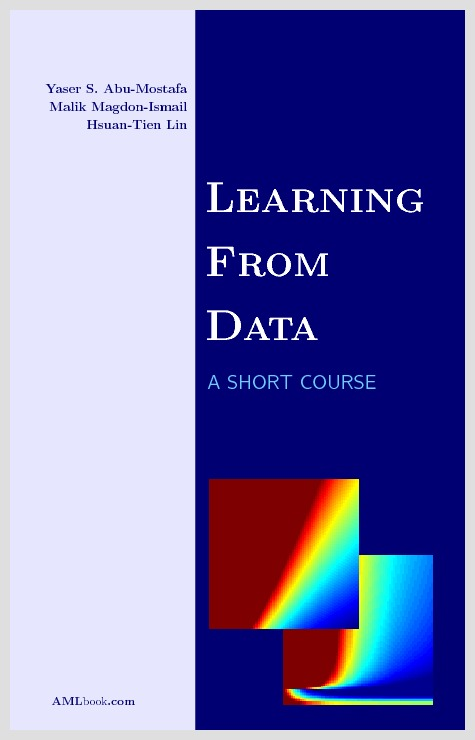
\includegraphics[width=2.5cm]{lfd.jpg}
        }
          \end{center}
        \end{column}
      \end{columns}
    \end{exampleblock}
    \vskip -.75em
    \begin{columns}
      \begin{column}{5.5cm}
        \begin{block}<5->{as machine learning researcher}
          machine learning \alert{for} big data\\ \onslide<6->
          ---easy?! \smileyface
        \end{block}
      \end{column}

      \begin{column}{5.5cm}
        \begin{alertblock}<7->{as machine learning educator}
          \alert{human} learning \alert{for} big data\\
          ---\alert{hard!!} \vphantom{\smileyface}
        \end{alertblock}
      \end{column}
    \end{columns}

    \vskip -.5em \onslide<8->
    \chint{
      will focus on \alert{human} learning \alert{for} big data
    }
  \end{frame}

  \begin{frame}
    \frametitle{Human Learning for Big Data}
    
    \begin{block}{Todo}
      \begin{itemize}
      \item<1-> some FAQs that I have encountered as 
        \begin{itemize}
        \item<2-> \alert{educator} (NTU and NTU@Coursera)
        \item<3-> \alert{team mentor} (KDDCups, TSMC Big Data competition, etc.)
        \item<4-> \alert{researcher} (CLLab@NTU)
        \item<5-> \alert{data scientist} (
\includegraphics[width=1cm]{appier.png}), a AI-based startup
        \end{itemize}
      \item<6-> my imperfect yet \alertblue{honest} answers
        that hint \alertblue{what shall be learned}
      \end{itemize}     
    \end{block}
    \vskip -.3em
    \begin{alertblock}<7->{First Honest Claims}
      \begin{itemize}
      \item<7-> must-learn for \alert{big data} $\approx$ must-learn for \alertblue{small data} in ML, \\
        \onslide<8-> but the former with \alert{bigger seriousness}
      \item<9-> system design/architecture \alert{very important}, \onslide<10->but somewhat beyond my pay grade
      \end{itemize}
    \end{alertblock}
    \vskip -1em \onslide<11->
    \chint{
      \textit{I wish I had an answer to that \\because I'm tired of answering that question.\\---Yogi Berra (Athlete)} \smileyface
    }
    
  \end{frame}


  \begin{frame}
    \frametitle{Appendix: ML Foundations on NTU@Coursera}

    \begin{block}{}
      \centering
      \url{https://www.coursera.org/course/ntumlone}
    \end{block}
    \vskip -.5em
    \begin{exampleblock}{}
      \small
      \begin{columns}
        \begin{column}{5.8cm}
        When can machines learn?
          \begin{itemize}
          \item L1: the learning problem (\smileyface)
          \item L2: learning to answer yes/no (\smileyface)
          \item L3: types of learning (\smileyface)
          \item L4: feasibility of learning
          \end{itemize}
        Why can machines learn?
          \begin{itemize}
          \item L5: training versus testing
          \item L6: theory of generalization
          \item L7: the VC dimension (\smileyface)
          \item L8: noise and error
          \end{itemize}
        \end{column}
        \begin{column}{6.2cm}
        How can machines learn?
          \begin{itemize}
          \item L9: linear regression (\smileyface)
          \item L10: logistic regression	(\smileyface)
          \item L11: linear models for classification (\smileyface)
          \item L12: nonlinear transformation (\smileyface)
          \end{itemize}
        How can machines learn better?
          \begin{itemize}
          \item L13: hazard of overfitting (\smileyface)
          \item L14: regularization (\smileyface)
          \item L15: validation (\smileyface)
          \item L16: three learning principles (\smileyface)
          \end{itemize}
        \end{column}
      \end{columns}
    \end{exampleblock}
    \vskip -1.2em
    \chint{
      \large \smileyface\ \ $\approx$ must-learn
    }
  \end{frame}
\end{CJK*}
\end{document}
